% System design and implementation of the live-call detector (owner SK).
% Referenced from main.tex as % System design and implementation of the live-call detector (owner SK).
% Referenced from main.tex as % System design and implementation of the live-call detector (owner SK).
% Referenced from main.tex as % System design and implementation of the live-call detector (owner SK).
% Referenced from main.tex as \input{sections/system}; label sec:system.
\section{System Design and Implementation}
\label{sec:system}

The evaluation protocol in Section~\ref{sec:method} scores four-second windows
of narrowband telephone audio. The deployed system is that protocol running on a
live call rather than on a manifest: the same encoder, the same windowing, the same
operating point. Nothing about the detector changes between the two, which is what
lets a demonstration stand as evidence rather than as illustration.

\subsection{Requirements}

Four requirements shaped the design, and each one rules out an otherwise obvious
implementation.

\textbf{The verdict must reach the callee and nobody else.} A system that tells the
caller they have been detected is a system that teaches attackers to evade it. This
is a routing requirement, and it is why call state is modelled explicitly rather
than broadcast to every participant of a session.

\textbf{The warning must arrive during the call.} A verdict delivered after the call
has ended protects nobody. This sets a latency budget rather than a throughput one:
the first credible warning must land within roughly ten seconds of speech.

\textbf{The audio the detector sees must be the audio it was trained on.} The
adapted model is trained on 8\,kHz G.711 telephone audio, and its decision cue lives
in fine waveform structure (Section~\ref{sec:results}). Any resampling, codec or
level change between the carrier and the model is a domain shift.

\textbf{A single false alarm is more damaging than a missed clone.} The user is a
person receiving a call from someone they may know. The escalation ladder below is
built around that asymmetry.

\subsection{Architecture}

The system is a single Python service with three layers: carriers, which turn a call
into a stream of audio frames; a detection core, which is carrier-agnostic; and
delivery, which routes verdicts to the right participant.

\begin{figure}[t]
  \centering
  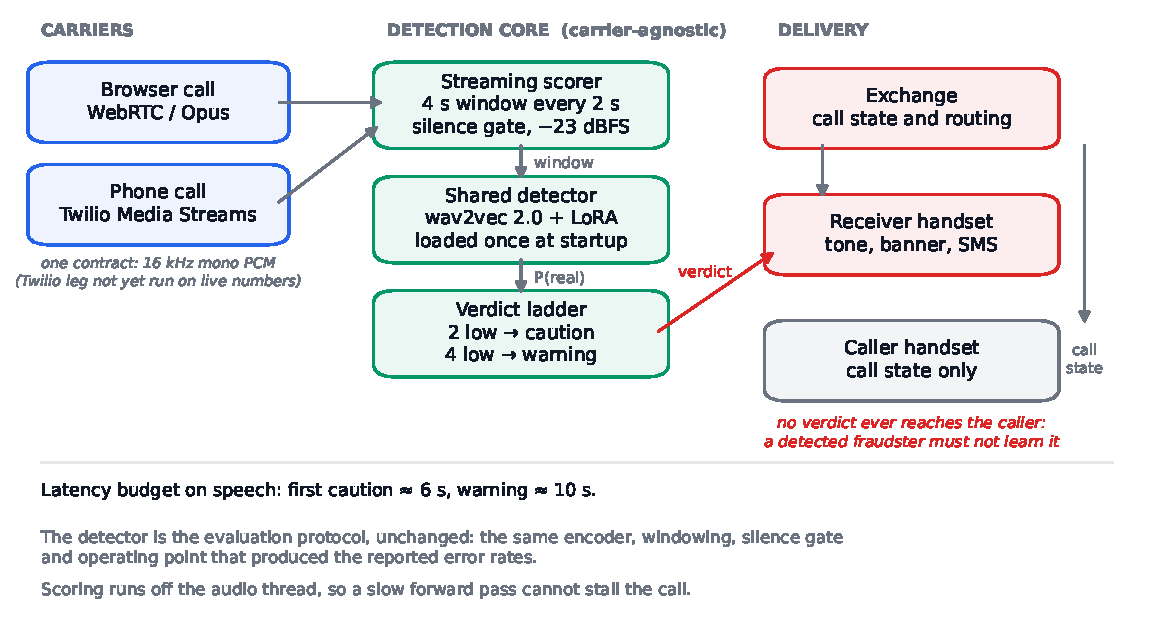
\includegraphics[width=\linewidth]{figures/system_architecture.pdf}
  \caption{The live-call detector. Two carriers, WebRTC and Twilio Media Streams,
  both resolve to the same 16\,kHz mono PCM contract, so the detection core is
  unaware of which one delivered the call. Verdicts travel only to the receiver's
  handset.}
  \label{fig:system}
\end{figure}

\subsubsection{Carriers}

Two carriers are implemented against one contract, a \texttt{PcmFrameSource} that
yields 16\,kHz mono float frames.

\emph{WebRTC} (\texttt{live\_call/webrtc\_harness/}) carries browser-to-browser
calls. The server is a participant in the call rather than a bystander: it accepts
an offer, subscribes to each peer's audio through a relay, and taps one copy for
detection while forwarding another to the other party. Audio tracks are keyed by
peer and dropped when that peer leaves; an earlier implementation accumulated every
past call's tracks in the room and eventually offered a new joiner more media lines
than its session description contained, which fails negotiation outright.

\emph{Twilio Media Streams} (\texttt{live\_call/media\_handler.py}) carries calls
from the public telephone network. Twilio opens a WebSocket and pushes base64
G.711 $\mu$-law at 8\,kHz; the handler decodes and resamples to the same contract.
Requests are authenticated by HMAC signature before any audio is accepted.

\subsubsection{Detection core}

One detector is shared by every call (\texttt{live\_call/detector.py}): the
checkpoint is loaded once at startup, not per call, because loading it inside the
first request added tens of seconds of silence to that call. Each call owns a
session (\texttt{live\_call/session.py}) that pulls frames, and the streaming scorer
(\texttt{src/inference/streaming.py}) applies the evaluation-time treatment: a
four-second window every two seconds, a $-50$\,dBFS silence gate so that pauses are
skipped rather than scored, and normalisation to $-23$\,dBFS.

Scoring happens on a worker thread. A slow forward pass must not stall the audio
path, because the carrier does not wait: frames arrive in real time whether or not
the previous window has finished.

\subsubsection{The escalation ladder}

A per-window score is too noisy to act on. The verdict engine
(\texttt{live\_call/verdict\_engine.py}) requires agreement across consecutive
windows before it escalates:

\begin{itemize}
  \item \textbf{Listening} until the first window is scored.
  \item \textbf{Suspicious} after two consecutive windows below the threshold: an
    audible tone and a caution on the receiver's handset.
  \item \textbf{Likely cloned} after four: a spoken warning to the receiver's leg of
    the call and, on the telephone carrier, an SMS.
  \item Recovery after three consecutive windows above the threshold, so a single
    noisy stretch does not leave a call marked for its duration.
\end{itemize}

With a two-second hop this places the first caution near six seconds of speech and
the warning near ten. The asymmetry is deliberate: four windows to accuse, three to
forgive.

\subsubsection{Call state and routing}

The exchange (\texttt{live\_call/phone.py}) models a line as
\emph{idle}, \emph{ringing}, \emph{connected} or \emph{ended}, with the parties on
it. It holds no sockets and no audio, which makes the routing rule testable in
isolation: verdicts are addressed to the receiver's connection only, and the
caller's connection receives call state alone.

Two consequences of this design are worth recording because both were found by
running real calls rather than by reasoning about the code. First, monitoring starts
when the call is \emph{answered}, not when the caller's audio arrives; during
ringing the media path is still settling, and the resulting discontinuity scored as
two low windows and cautioned a genuine caller. Second, the receiver's audio path is
opened while the phone is ringing, so that the renegotiation it triggers completes
before anyone speaks.

\subsection{Interfaces}

A browser-based console presents both handsets, the signal path and the live
analysis on one screen; separate caller and receiver pages run the same code on two
devices. A dashboard exposes every scored window for inspection. The evaluation
endpoints (\texttt{/api/predict}, \texttt{/api/replay}) score a file through the
identical path, which is how the operating point was calibrated and how the
demonstration clips were verified.

\subsection{Verification}

The system is covered at three levels. Unit tests cover the exchange, the verdict
ladder, the windowing and the room bookkeeping. Integration tests drive the real
sockets. End-to-end tests place calls in a real browser against the loaded model and
assert the properties that matter: that a cloned caller raises the warning within
the budget, that a genuine caller raises nothing, that every two seconds of speech
produces a scored window, and that no verdict ever appears on the caller's side.

That last layer exists because the defects that mattered were all in the wiring
between components that each worked correctly alone. The most serious example: the
alert message carries its severity in one field and its delivery channel in another,
and the interface read the channel. Every unit test passed, the ladder escalated
correctly, the message was dispatched --- and no warning was ever displayed.

\subsection{Deployment status}

The WebRTC carrier is verified end to end against the deployed checkpoint. Each
demonstration clip was replayed through the live path and its behaviour recorded
rather than inferred from offline scores, because the two disagree: on a live call a
genuine caller can lose several consecutive windows that the same clip never loses
offline.

We tested the obvious explanation and it does not hold. Encoding each clip through
the browser's carrier offline --- resample to 48\,kHz, Opus encode and decode,
resample back --- and rescoring through the identical streaming path leaves both
genuine clips at zero windows below the threshold, with a worst window of 0.984
against the 0.001 seen live. Both seen attacks stay fully detected through every
carrier. The codec, and the resampling around it, therefore do not account for the
live degradation, and clone detection does not depend on codec artefacts.\footnote{%
\texttt{docs/results/carrier\_effect\_v1.md}; reproduce with
\texttt{python -m src.inference.carrier\_sim}.}

By elimination the cause lies in the real-time transport rather than in the coding:
jitter buffering, packet-loss concealment, or the bitrate adaptation a browser
applies while a connection is still settling. Concealment is the candidate we would
test first, because it synthesises audio to fill gaps, and a detector reporting that
machine-generated audio is not human would produce exactly this signature. That
remains untested. The call is negotiated at a high constant bitrate with
discontinuous transmission disabled, which is sensible for a demonstration, but the
dip survived that change and it should not be presented as the remedy.

The Twilio carrier is implemented and unit-tested but has not been verified on live
numbers, because the account's trial credit was exhausted. This is the clearest
piece of remaining work: the protocol the system was designed around is the
telephone network, and the telephone leg is the one leg not yet demonstrated.
; label sec:system.
\section{System Design and Implementation}
\label{sec:system}

The evaluation protocol in Section~\ref{sec:method} scores four-second windows
of narrowband telephone audio. The deployed system is that protocol running on a
live call rather than on a manifest: the same encoder, the same windowing, the same
operating point. Nothing about the detector changes between the two, which is what
lets a demonstration stand as evidence rather than as illustration.

\subsection{Requirements}

Four requirements shaped the design, and each one rules out an otherwise obvious
implementation.

\textbf{The verdict must reach the callee and nobody else.} A system that tells the
caller they have been detected is a system that teaches attackers to evade it. This
is a routing requirement, and it is why call state is modelled explicitly rather
than broadcast to every participant of a session.

\textbf{The warning must arrive during the call.} A verdict delivered after the call
has ended protects nobody. This sets a latency budget rather than a throughput one:
the first credible warning must land within roughly ten seconds of speech.

\textbf{The audio the detector sees must be the audio it was trained on.} The
adapted model is trained on 8\,kHz G.711 telephone audio, and its decision cue lives
in fine waveform structure (Section~\ref{sec:results}). Any resampling, codec or
level change between the carrier and the model is a domain shift.

\textbf{A single false alarm is more damaging than a missed clone.} The user is a
person receiving a call from someone they may know. The escalation ladder below is
built around that asymmetry.

\subsection{Architecture}

The system is a single Python service with three layers: carriers, which turn a call
into a stream of audio frames; a detection core, which is carrier-agnostic; and
delivery, which routes verdicts to the right participant.

\begin{figure}[t]
  \centering
  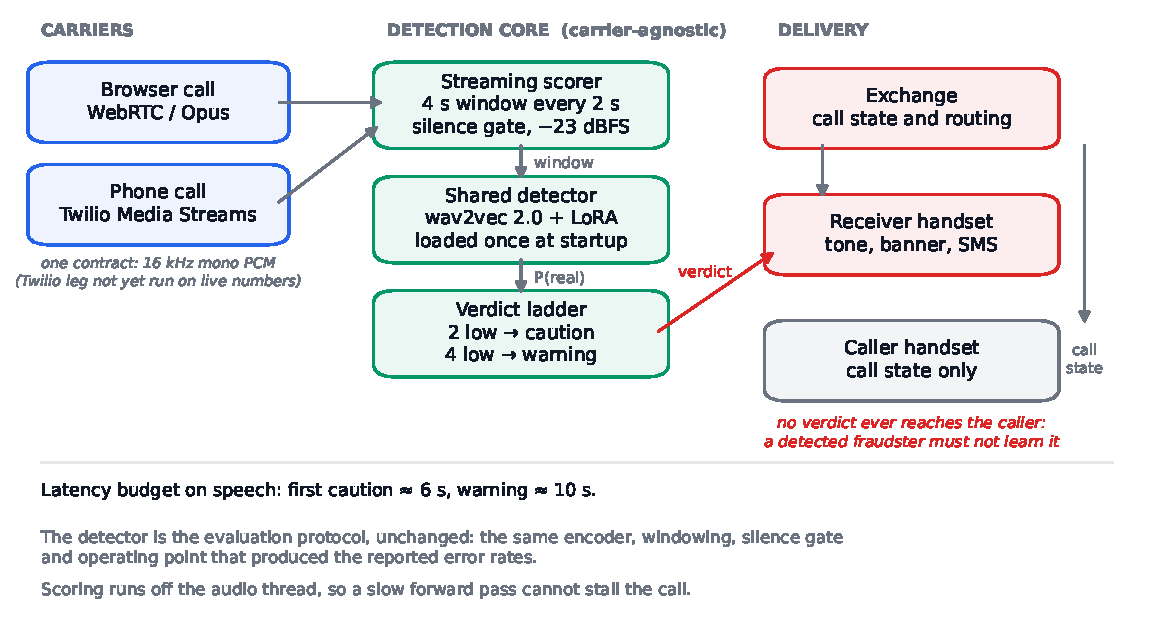
\includegraphics[width=\linewidth]{figures/system_architecture.pdf}
  \caption{The live-call detector. Two carriers, WebRTC and Twilio Media Streams,
  both resolve to the same 16\,kHz mono PCM contract, so the detection core is
  unaware of which one delivered the call. Verdicts travel only to the receiver's
  handset.}
  \label{fig:system}
\end{figure}

\subsubsection{Carriers}

Two carriers are implemented against one contract, a \texttt{PcmFrameSource} that
yields 16\,kHz mono float frames.

\emph{WebRTC} (\texttt{live\_call/webrtc\_harness/}) carries browser-to-browser
calls. The server is a participant in the call rather than a bystander: it accepts
an offer, subscribes to each peer's audio through a relay, and taps one copy for
detection while forwarding another to the other party. Audio tracks are keyed by
peer and dropped when that peer leaves; an earlier implementation accumulated every
past call's tracks in the room and eventually offered a new joiner more media lines
than its session description contained, which fails negotiation outright.

\emph{Twilio Media Streams} (\texttt{live\_call/media\_handler.py}) carries calls
from the public telephone network. Twilio opens a WebSocket and pushes base64
G.711 $\mu$-law at 8\,kHz; the handler decodes and resamples to the same contract.
Requests are authenticated by HMAC signature before any audio is accepted.

\subsubsection{Detection core}

One detector is shared by every call (\texttt{live\_call/detector.py}): the
checkpoint is loaded once at startup, not per call, because loading it inside the
first request added tens of seconds of silence to that call. Each call owns a
session (\texttt{live\_call/session.py}) that pulls frames, and the streaming scorer
(\texttt{src/inference/streaming.py}) applies the evaluation-time treatment: a
four-second window every two seconds, a $-50$\,dBFS silence gate so that pauses are
skipped rather than scored, and normalisation to $-23$\,dBFS.

Scoring happens on a worker thread. A slow forward pass must not stall the audio
path, because the carrier does not wait: frames arrive in real time whether or not
the previous window has finished.

\subsubsection{The escalation ladder}

A per-window score is too noisy to act on. The verdict engine
(\texttt{live\_call/verdict\_engine.py}) requires agreement across consecutive
windows before it escalates:

\begin{itemize}
  \item \textbf{Listening} until the first window is scored.
  \item \textbf{Suspicious} after two consecutive windows below the threshold: an
    audible tone and a caution on the receiver's handset.
  \item \textbf{Likely cloned} after four: a spoken warning to the receiver's leg of
    the call and, on the telephone carrier, an SMS.
  \item Recovery after three consecutive windows above the threshold, so a single
    noisy stretch does not leave a call marked for its duration.
\end{itemize}

With a two-second hop this places the first caution near six seconds of speech and
the warning near ten. The asymmetry is deliberate: four windows to accuse, three to
forgive.

\subsubsection{Call state and routing}

The exchange (\texttt{live\_call/phone.py}) models a line as
\emph{idle}, \emph{ringing}, \emph{connected} or \emph{ended}, with the parties on
it. It holds no sockets and no audio, which makes the routing rule testable in
isolation: verdicts are addressed to the receiver's connection only, and the
caller's connection receives call state alone.

Two consequences of this design are worth recording because both were found by
running real calls rather than by reasoning about the code. First, monitoring starts
when the call is \emph{answered}, not when the caller's audio arrives; during
ringing the media path is still settling, and the resulting discontinuity scored as
two low windows and cautioned a genuine caller. Second, the receiver's audio path is
opened while the phone is ringing, so that the renegotiation it triggers completes
before anyone speaks.

\subsection{Interfaces}

A browser-based console presents both handsets, the signal path and the live
analysis on one screen; separate caller and receiver pages run the same code on two
devices. A dashboard exposes every scored window for inspection. The evaluation
endpoints (\texttt{/api/predict}, \texttt{/api/replay}) score a file through the
identical path, which is how the operating point was calibrated and how the
demonstration clips were verified.

\subsection{Verification}

The system is covered at three levels. Unit tests cover the exchange, the verdict
ladder, the windowing and the room bookkeeping. Integration tests drive the real
sockets. End-to-end tests place calls in a real browser against the loaded model and
assert the properties that matter: that a cloned caller raises the warning within
the budget, that a genuine caller raises nothing, that every two seconds of speech
produces a scored window, and that no verdict ever appears on the caller's side.

That last layer exists because the defects that mattered were all in the wiring
between components that each worked correctly alone. The most serious example: the
alert message carries its severity in one field and its delivery channel in another,
and the interface read the channel. Every unit test passed, the ladder escalated
correctly, the message was dispatched --- and no warning was ever displayed.

\subsection{Deployment status}

The WebRTC carrier is verified end to end against the deployed checkpoint. Each
demonstration clip was replayed through the live path and its behaviour recorded
rather than inferred from offline scores, because the two disagree: on a live call a
genuine caller can lose several consecutive windows that the same clip never loses
offline.

We tested the obvious explanation and it does not hold. Encoding each clip through
the browser's carrier offline --- resample to 48\,kHz, Opus encode and decode,
resample back --- and rescoring through the identical streaming path leaves both
genuine clips at zero windows below the threshold, with a worst window of 0.984
against the 0.001 seen live. Both seen attacks stay fully detected through every
carrier. The codec, and the resampling around it, therefore do not account for the
live degradation, and clone detection does not depend on codec artefacts.\footnote{%
\texttt{docs/results/carrier\_effect\_v1.md}; reproduce with
\texttt{python -m src.inference.carrier\_sim}.}

By elimination the cause lies in the real-time transport rather than in the coding:
jitter buffering, packet-loss concealment, or the bitrate adaptation a browser
applies while a connection is still settling. Concealment is the candidate we would
test first, because it synthesises audio to fill gaps, and a detector reporting that
machine-generated audio is not human would produce exactly this signature. That
remains untested. The call is negotiated at a high constant bitrate with
discontinuous transmission disabled, which is sensible for a demonstration, but the
dip survived that change and it should not be presented as the remedy.

The Twilio carrier is implemented and unit-tested but has not been verified on live
numbers, because the account's trial credit was exhausted. This is the clearest
piece of remaining work: the protocol the system was designed around is the
telephone network, and the telephone leg is the one leg not yet demonstrated.
; label sec:system.
\section{System Design and Implementation}
\label{sec:system}

The evaluation protocol in Section~\ref{sec:method} scores four-second windows
of narrowband telephone audio. The deployed system is that protocol running on a
live call rather than on a manifest: the same encoder, the same windowing, the same
operating point. Nothing about the detector changes between the two, which is what
lets a demonstration stand as evidence rather than as illustration.

\subsection{Requirements}

Four requirements shaped the design, and each one rules out an otherwise obvious
implementation.

\textbf{The verdict must reach the callee and nobody else.} A system that tells the
caller they have been detected is a system that teaches attackers to evade it. This
is a routing requirement, and it is why call state is modelled explicitly rather
than broadcast to every participant of a session.

\textbf{The warning must arrive during the call.} A verdict delivered after the call
has ended protects nobody. This sets a latency budget rather than a throughput one:
the first credible warning must land within roughly ten seconds of speech.

\textbf{The audio the detector sees must be the audio it was trained on.} The
adapted model is trained on 8\,kHz G.711 telephone audio, and its decision cue lives
in fine waveform structure (Section~\ref{sec:results}). Any resampling, codec or
level change between the carrier and the model is a domain shift.

\textbf{A single false alarm is more damaging than a missed clone.} The user is a
person receiving a call from someone they may know. The escalation ladder below is
built around that asymmetry.

\subsection{Architecture}

The system is a single Python service with three layers: carriers, which turn a call
into a stream of audio frames; a detection core, which is carrier-agnostic; and
delivery, which routes verdicts to the right participant.

\begin{figure}[t]
  \centering
  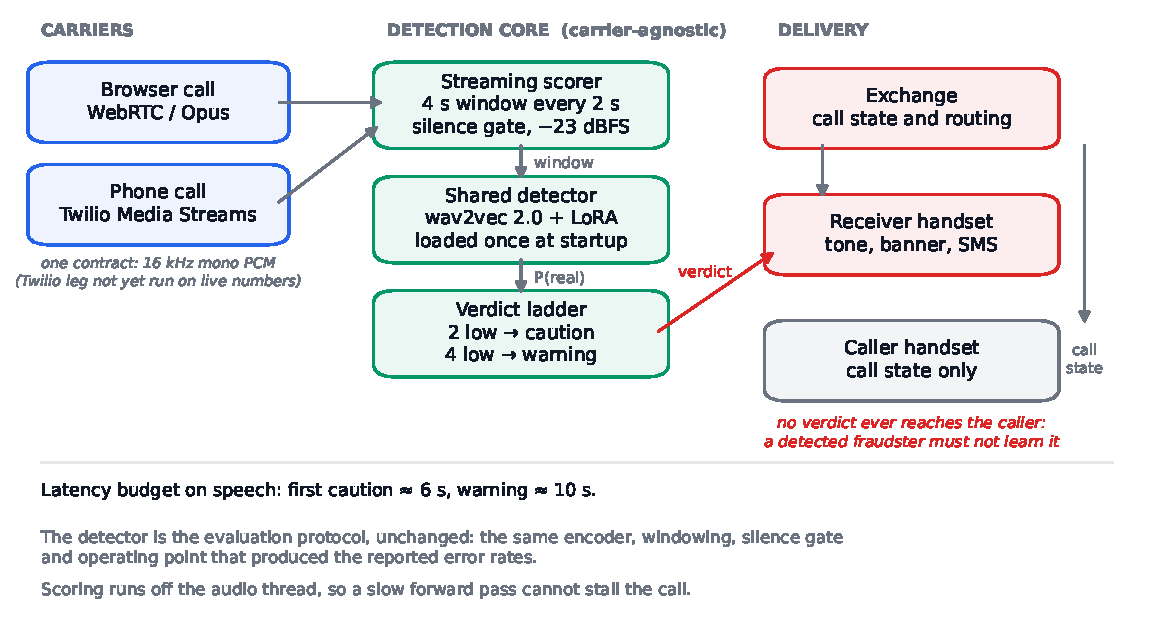
\includegraphics[width=\linewidth]{figures/system_architecture.pdf}
  \caption{The live-call detector. Two carriers, WebRTC and Twilio Media Streams,
  both resolve to the same 16\,kHz mono PCM contract, so the detection core is
  unaware of which one delivered the call. Verdicts travel only to the receiver's
  handset.}
  \label{fig:system}
\end{figure}

\subsubsection{Carriers}

Two carriers are implemented against one contract, a \texttt{PcmFrameSource} that
yields 16\,kHz mono float frames.

\emph{WebRTC} (\texttt{live\_call/webrtc\_harness/}) carries browser-to-browser
calls. The server is a participant in the call rather than a bystander: it accepts
an offer, subscribes to each peer's audio through a relay, and taps one copy for
detection while forwarding another to the other party. Audio tracks are keyed by
peer and dropped when that peer leaves; an earlier implementation accumulated every
past call's tracks in the room and eventually offered a new joiner more media lines
than its session description contained, which fails negotiation outright.

\emph{Twilio Media Streams} (\texttt{live\_call/media\_handler.py}) carries calls
from the public telephone network. Twilio opens a WebSocket and pushes base64
G.711 $\mu$-law at 8\,kHz; the handler decodes and resamples to the same contract.
Requests are authenticated by HMAC signature before any audio is accepted.

\subsubsection{Detection core}

One detector is shared by every call (\texttt{live\_call/detector.py}): the
checkpoint is loaded once at startup, not per call, because loading it inside the
first request added tens of seconds of silence to that call. Each call owns a
session (\texttt{live\_call/session.py}) that pulls frames, and the streaming scorer
(\texttt{src/inference/streaming.py}) applies the evaluation-time treatment: a
four-second window every two seconds, a $-50$\,dBFS silence gate so that pauses are
skipped rather than scored, and normalisation to $-23$\,dBFS.

Scoring happens on a worker thread. A slow forward pass must not stall the audio
path, because the carrier does not wait: frames arrive in real time whether or not
the previous window has finished.

\subsubsection{The escalation ladder}

A per-window score is too noisy to act on. The verdict engine
(\texttt{live\_call/verdict\_engine.py}) requires agreement across consecutive
windows before it escalates:

\begin{itemize}
  \item \textbf{Listening} until the first window is scored.
  \item \textbf{Suspicious} after two consecutive windows below the threshold: an
    audible tone and a caution on the receiver's handset.
  \item \textbf{Likely cloned} after four: a spoken warning to the receiver's leg of
    the call and, on the telephone carrier, an SMS.
  \item Recovery after three consecutive windows above the threshold, so a single
    noisy stretch does not leave a call marked for its duration.
\end{itemize}

With a two-second hop this places the first caution near six seconds of speech and
the warning near ten. The asymmetry is deliberate: four windows to accuse, three to
forgive.

\subsubsection{Call state and routing}

The exchange (\texttt{live\_call/phone.py}) models a line as
\emph{idle}, \emph{ringing}, \emph{connected} or \emph{ended}, with the parties on
it. It holds no sockets and no audio, which makes the routing rule testable in
isolation: verdicts are addressed to the receiver's connection only, and the
caller's connection receives call state alone.

Two consequences of this design are worth recording because both were found by
running real calls rather than by reasoning about the code. First, monitoring starts
when the call is \emph{answered}, not when the caller's audio arrives; during
ringing the media path is still settling, and the resulting discontinuity scored as
two low windows and cautioned a genuine caller. Second, the receiver's audio path is
opened while the phone is ringing, so that the renegotiation it triggers completes
before anyone speaks.

\subsection{Interfaces}

A browser-based console presents both handsets, the signal path and the live
analysis on one screen; separate caller and receiver pages run the same code on two
devices. A dashboard exposes every scored window for inspection. The evaluation
endpoints (\texttt{/api/predict}, \texttt{/api/replay}) score a file through the
identical path, which is how the operating point was calibrated and how the
demonstration clips were verified.

\subsection{Verification}

The system is covered at three levels. Unit tests cover the exchange, the verdict
ladder, the windowing and the room bookkeeping. Integration tests drive the real
sockets. End-to-end tests place calls in a real browser against the loaded model and
assert the properties that matter: that a cloned caller raises the warning within
the budget, that a genuine caller raises nothing, that every two seconds of speech
produces a scored window, and that no verdict ever appears on the caller's side.

That last layer exists because the defects that mattered were all in the wiring
between components that each worked correctly alone. The most serious example: the
alert message carries its severity in one field and its delivery channel in another,
and the interface read the channel. Every unit test passed, the ladder escalated
correctly, the message was dispatched --- and no warning was ever displayed.

\subsection{Deployment status}

The WebRTC carrier is verified end to end against the deployed checkpoint. Each
demonstration clip was replayed through the live path and its behaviour recorded
rather than inferred from offline scores, because the two disagree: on a live call a
genuine caller can lose several consecutive windows that the same clip never loses
offline.

We tested the obvious explanation and it does not hold. Encoding each clip through
the browser's carrier offline --- resample to 48\,kHz, Opus encode and decode,
resample back --- and rescoring through the identical streaming path leaves both
genuine clips at zero windows below the threshold, with a worst window of 0.984
against the 0.001 seen live. Both seen attacks stay fully detected through every
carrier. The codec, and the resampling around it, therefore do not account for the
live degradation, and clone detection does not depend on codec artefacts.\footnote{%
\texttt{docs/results/carrier\_effect\_v1.md}; reproduce with
\texttt{python -m src.inference.carrier\_sim}.}

By elimination the cause lies in the real-time transport rather than in the coding:
jitter buffering, packet-loss concealment, or the bitrate adaptation a browser
applies while a connection is still settling. Concealment is the candidate we would
test first, because it synthesises audio to fill gaps, and a detector reporting that
machine-generated audio is not human would produce exactly this signature. That
remains untested. The call is negotiated at a high constant bitrate with
discontinuous transmission disabled, which is sensible for a demonstration, but the
dip survived that change and it should not be presented as the remedy.

The Twilio carrier is implemented and unit-tested but has not been verified on live
numbers, because the account's trial credit was exhausted. This is the clearest
piece of remaining work: the protocol the system was designed around is the
telephone network, and the telephone leg is the one leg not yet demonstrated.
; label sec:system.
\section{System Design and Implementation}
\label{sec:system}

The evaluation protocol in Section~\ref{sec:method} scores four-second windows
of narrowband telephone audio. The deployed system is that protocol running on a
live call rather than on a manifest: the same encoder, the same windowing, the same
operating point. Nothing about the detector changes between the two, which is what
lets a demonstration stand as evidence rather than as illustration.

\subsection{Requirements}

Four requirements shaped the design, and each one rules out an otherwise obvious
implementation.

\textbf{The verdict must reach the callee and nobody else.} A system that tells the
caller they have been detected is a system that teaches attackers to evade it. This
is a routing requirement, and it is why call state is modelled explicitly rather
than broadcast to every participant of a session.

\textbf{The warning must arrive during the call.} A verdict delivered after the call
has ended protects nobody. This sets a latency budget rather than a throughput one:
the first credible warning must land within roughly ten seconds of speech.

\textbf{The audio the detector sees must be the audio it was trained on.} The
adapted model is trained on 8\,kHz G.711 telephone audio, and its decision cue lives
in fine waveform structure (Section~\ref{sec:results}). Any resampling, codec or
level change between the carrier and the model is a domain shift.

\textbf{A single false alarm is more damaging than a missed clone.} The user is a
person receiving a call from someone they may know. The escalation ladder below is
built around that asymmetry.

\subsection{Architecture}

The system is a single Python service with three layers: carriers, which turn a call
into a stream of audio frames; a detection core, which is carrier-agnostic; and
delivery, which routes verdicts to the right participant.

\begin{figure}[t]
  \centering
  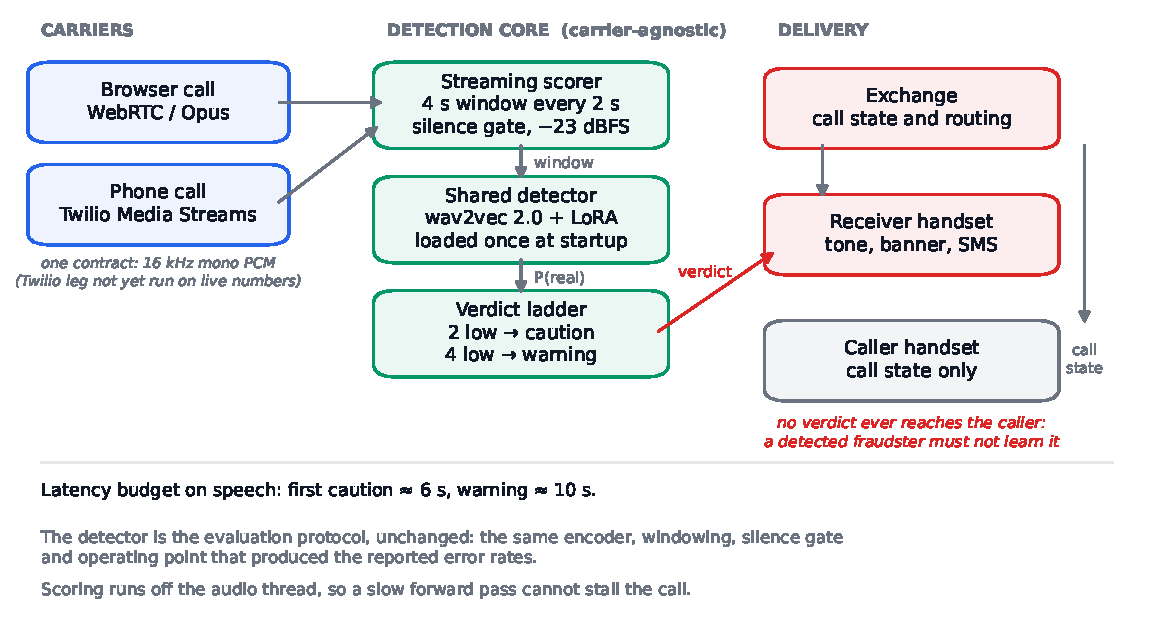
\includegraphics[width=\linewidth]{figures/system_architecture.pdf}
  \caption{The live-call detector. Two carriers, WebRTC and Twilio Media Streams,
  both resolve to the same 16\,kHz mono PCM contract, so the detection core is
  unaware of which one delivered the call. Verdicts travel only to the receiver's
  handset.}
  \label{fig:system}
\end{figure}

\subsubsection{Carriers}

Two carriers are implemented against one contract, a \texttt{PcmFrameSource} that
yields 16\,kHz mono float frames.

\emph{WebRTC} (\texttt{live\_call/webrtc\_harness/}) carries browser-to-browser
calls. The server is a participant in the call rather than a bystander: it accepts
an offer, subscribes to each peer's audio through a relay, and taps one copy for
detection while forwarding another to the other party. Audio tracks are keyed by
peer and dropped when that peer leaves; an earlier implementation accumulated every
past call's tracks in the room and eventually offered a new joiner more media lines
than its session description contained, which fails negotiation outright.

\emph{Twilio Media Streams} (\texttt{live\_call/media\_handler.py}) carries calls
from the public telephone network. Twilio opens a WebSocket and pushes base64
G.711 $\mu$-law at 8\,kHz; the handler decodes and resamples to the same contract.
Requests are authenticated by HMAC signature before any audio is accepted.

\subsubsection{Detection core}

One detector is shared by every call (\texttt{live\_call/detector.py}): the
checkpoint is loaded once at startup, not per call, because loading it inside the
first request added tens of seconds of silence to that call. Each call owns a
session (\texttt{live\_call/session.py}) that pulls frames, and the streaming scorer
(\texttt{src/inference/streaming.py}) applies the evaluation-time treatment: a
four-second window every two seconds, a $-50$\,dBFS silence gate so that pauses are
skipped rather than scored, and normalisation to $-23$\,dBFS.

Scoring happens on a worker thread. A slow forward pass must not stall the audio
path, because the carrier does not wait: frames arrive in real time whether or not
the previous window has finished.

\subsubsection{The escalation ladder}

A per-window score is too noisy to act on. The verdict engine
(\texttt{live\_call/verdict\_engine.py}) requires agreement across consecutive
windows before it escalates:

\begin{itemize}
  \item \textbf{Listening} until the first window is scored.
  \item \textbf{Suspicious} after two consecutive windows below the threshold: an
    audible tone and a caution on the receiver's handset.
  \item \textbf{Likely cloned} after four: a spoken warning to the receiver's leg of
    the call and, on the telephone carrier, an SMS.
  \item Recovery after three consecutive windows above the threshold, so a single
    noisy stretch does not leave a call marked for its duration.
\end{itemize}

With a two-second hop this places the first caution near six seconds of speech and
the warning near ten. The asymmetry is deliberate: four windows to accuse, three to
forgive.

\subsubsection{Call state and routing}

The exchange (\texttt{live\_call/phone.py}) models a line as
\emph{idle}, \emph{ringing}, \emph{connected} or \emph{ended}, with the parties on
it. It holds no sockets and no audio, which makes the routing rule testable in
isolation: verdicts are addressed to the receiver's connection only, and the
caller's connection receives call state alone.

Two consequences of this design are worth recording because both were found by
running real calls rather than by reasoning about the code. First, monitoring starts
when the call is \emph{answered}, not when the caller's audio arrives; during
ringing the media path is still settling, and the resulting discontinuity scored as
two low windows and cautioned a genuine caller. Second, the receiver's audio path is
opened while the phone is ringing, so that the renegotiation it triggers completes
before anyone speaks.

\subsection{Interfaces}

A browser-based console presents both handsets, the signal path and the live
analysis on one screen; separate caller and receiver pages run the same code on two
devices. A dashboard exposes every scored window for inspection. The evaluation
endpoints (\texttt{/api/predict}, \texttt{/api/replay}) score a file through the
identical path, which is how the operating point was calibrated and how the
demonstration clips were verified.

\subsection{Verification}

The system is covered at three levels. Unit tests cover the exchange, the verdict
ladder, the windowing and the room bookkeeping. Integration tests drive the real
sockets. End-to-end tests place calls in a real browser against the loaded model and
assert the properties that matter: that a cloned caller raises the warning within
the budget, that a genuine caller raises nothing, that every two seconds of speech
produces a scored window, and that no verdict ever appears on the caller's side.

That last layer exists because the defects that mattered were all in the wiring
between components that each worked correctly alone. The most serious example: the
alert message carries its severity in one field and its delivery channel in another,
and the interface read the channel. Every unit test passed, the ladder escalated
correctly, the message was dispatched --- and no warning was ever displayed.

\subsection{Deployment status}

The WebRTC carrier is verified end to end against the deployed checkpoint. Each
demonstration clip was replayed through the live path and its behaviour recorded
rather than inferred from offline scores, because the two disagree: on a live call a
genuine caller can lose several consecutive windows that the same clip never loses
offline.

We tested the obvious explanation and it does not hold. Encoding each clip through
the browser's carrier offline --- resample to 48\,kHz, Opus encode and decode,
resample back --- and rescoring through the identical streaming path leaves both
genuine clips at zero windows below the threshold, with a worst window of 0.984
against the 0.001 seen live. Both seen attacks stay fully detected through every
carrier. The codec, and the resampling around it, therefore do not account for the
live degradation, and clone detection does not depend on codec artefacts.\footnote{%
\texttt{docs/results/carrier\_effect\_v1.md}; reproduce with
\texttt{python -m src.inference.carrier\_sim}.}

By elimination the cause lies in the real-time transport rather than in the coding:
jitter buffering, packet-loss concealment, or the bitrate adaptation a browser
applies while a connection is still settling. Concealment is the candidate we would
test first, because it synthesises audio to fill gaps, and a detector reporting that
machine-generated audio is not human would produce exactly this signature. That
remains untested. The call is negotiated at a high constant bitrate with
discontinuous transmission disabled, which is sensible for a demonstration, but the
dip survived that change and it should not be presented as the remedy.

The Twilio carrier is implemented and unit-tested but has not been verified on live
numbers, because the account's trial credit was exhausted. This is the clearest
piece of remaining work: the protocol the system was designed around is the
telephone network, and the telephone leg is the one leg not yet demonstrated.
